\section{Einleitung} % (fold)
\label{sec:einleitung}
	In diesem Versuch werden Funktionsweise und Kenngr"o"sen des Geiger-M"uller-Z"ahlrohrs untersucht.
	Das Ger"at erm"oglicht die Messung der Intensit"at ionisierender Strahlung.
	Auf Grund des einfachen Aufbaus ist das Geiger-M"uller-Z"ahlrohr kosteng"unstig und wegen seiner Verbreitung besonders interessant.

\section{Theorie} % (fold)
\label{sec:theorie}
	Zun"achst soll die Funktionsweise grob beschrieben werden.

	\subsection{Aufbau}
	\label{subsec:aufbau}
		Das Instrument besteht aus einem Anodendraht, der von einem Kathodenzylinder umschlossen ist.
		Der Raum zwischen Draht und Zylinder ist mit einem Gasgemisch niedrigend Drucks gef"ullt, das sich leicht ionisieren l"asst.
		Es wird eine Spannung $U$ zwischen $\SI{300}{\volt}$ und $\SI{2000}{\volt}$ an Anode und Kathode angelegt, wodurch ein radialsymmetrisches Feld im Innern des Zylinders entsteht.
		Der Zylinder ist von einem Stahlmantel umgeben, wobei eine Stirnseite aus einer d"unnen Membran aus Mylar besteht.
		Hierdurch wird m"oglichst wenig Strahlung beim Eintritt absorbiert und Gleichzeitig der Niederdruck im Inneren des Z"ahlrohrs bewahrt.

		\begin{figure}[h]
			\centering
			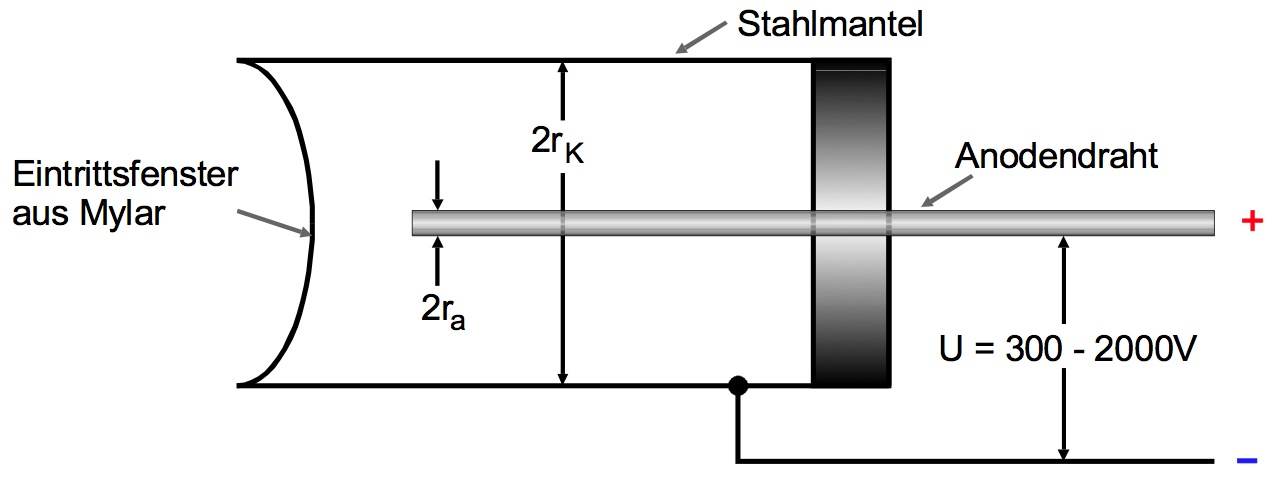
\includegraphics[width = 15cm]{img/zaehlrohr.jpeg}
			\caption{Querschnitt des Geiger-M"uller-Z"ahlrors}
			\label{fig:querschnitt}
		\end{figure}

	\subsection{Funktionsweise}
	\label{subsec:funktionsweise}
		Wenn ein geladenes Teilchen in das Z"ahlrohr eintritt, gibt es seine Energie an die Gasatome ab und kann diese ioniseren, bis seine Energie aufgebraucht ist.
		Weil die Energie des einfallenden Teilchens wesentlich gr"o"ser ist, als die zur Ionisation ben"otigte Energie, ist die Anzahl ionisierter Kerne proportional zur Energie des Teilchens.
		Die freigesetzten Gas-Ionen werden nun durch das elektrische Feld abgelenkt und bei gen"ugend gro"ser Spannung $U$ in Anode und Kathode absorbiert.
		Die Verschiedenen Wirkungsbereiche werden im Folgenden erl"autert.

		\begin{figure}[h]
			\centering
			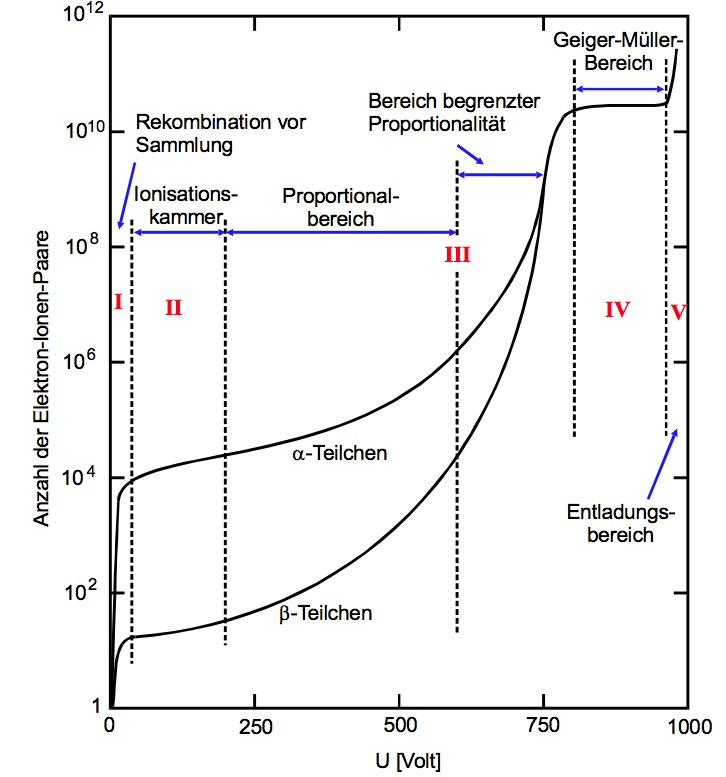
\includegraphics[width = 10cm]{img/bereiche.jpeg}
			\caption{Wirkungsbereiche des Geiger-M"uller-Z"ahlrohrs}
			\label{fig:bereiche}
		\end{figure}

		\subsubsection{Rekombination (I)}
		\label{subsubsec:rekombination}
			Bei zu geringer angelegter Spannung (beim vorliegenden Ger"at $U < \SI{300}{\volt}$) reicht die Feldst"arke im Zylinder nicht aus, um die Ionen vollst"andig zu trennen.
			Sie rekombinieren und die einfallende Strahlung l"asst sich nicht detektieren.

		\subsubsection{Ionisationskammer (II)}
		\label{subsubsec:ionisationskammer}
			Erh"oht man die Spannung, wird jedes ionisierte Molek"ul absorbiert und der Strom zwischen Anode und Kathode ist proportional zur Energie und zur Intensit"at der einfallenden Strahlung.
			Da der auftretende Strom jedoch sehr gering ist, kann nur Strahlung hoher Intensit"at gemessen werden.
			Man bezeichnet das Z"ahlrohr dann als Ionisationskammer.

		\subsubsection{Proportionalit"atsbereich (III)}
		\label{subsubsec:proportionalitaetsbereich}
			Bei gr"o"serer Spannung haben die im Zylinder freigestzten Elektronen gen"ugend Energie, um ihrerseits Molek"ule zu ionisieren.
			Auf diese Weise werden immer mehr Elektronen frei und man spricht man von einer \textsc{Townsend-Lawine}.
			Die Anzahl der freigesetzten Elektronen ist dabei nahezu proportional zur Energie der einfallenden Teilchen und die Spannung ist messbar gro"s.
			In diesem Bereich arbeitet der Detektor als Proportionalit"atsz"ahlrohr.

		\subsubsection{Geiger-M"uller-Bereich (IV)}
		\label{subsubsec:geiger-mueller-bereich}
			Wird die Spannung weiter erh"oht, entsteht bei den ersten Ionisationen eine Vielzahl von UV-Photonen, die sich im gesamten Z"ahlrohr ausbreiten und neue Elektronenlawinen ausl"osen.
			Die Ladung, die sich auf der Anode ansammelt ist dann unabh"angig von der Energie des einfallenden Teilchens.
			Dieser Spannungsbereich wird auch als Ausl"osebereich bezeichnet und ist die haupts"achliche Verwendungsart des Geiger-M"uller-Z"ahlrohrs.
			Die Anzahl der gemessenen Teilchen ist hier nahezu Konstant.
			Das so entstehende Plateau beschreibt die Charakteristik des Z"ahlrohrs.
			Ein langes Plateau mit geringer Steigung bedeutet dabei ein hochwertiges Z"ahlrohr.

			Bei noch h"ohren Spannungen wird durch ein einzelnes einfallendes Teilchen eine Dauerentladung gez"undet, wobei der anfallende Strom so schlie"slich stark wird, dass das Ger"at zerst"ort werden kann.

	\subsection{Nebeneffekte: Totzeit und Nachentladungen}
	\label{subsec:nebeneffekte}
		Ein unerw"unschter Effekt des Geiger-M"uller-Z"ahlrohrs wird als Totzeit bezeichnet.
		Weil die positiv geladenen Atomr"umpfe langsamer von der Kathode absorbiert werden, als die leichten Elektronen, bilden die R"umpfe f"ur eine Kurze zeit eine Ladungswolke, die dem elektrischen Feld entgegenwirkt.
		Dies macht weitere Ionisation unm"oglich.

		Zudem werden bei der Absorption der Atomr"umpfe in der Zylinderh"ulle m"oglicherweise Elektronen herausgeschlagen.
		Diese durchlaufen das gesamte Potential und k"onnen wiederum eine Lawine und damit einen messbaren Spannungsimpuls hervorrufen, der das Ergebnis verf"alscht.
		Diesem als Nachentladung bezeichneten Effekt wird durch zugabe von Alkohol-Gas entgegengewirkt.

	\subsection{Ansprechverm"ogen}
	\label{subsec:ansprechvermoegen}
		Das Ansprechverm"ogen bezeichnet die Wahrscheinlichkeit, mit der ein Teilchen detektiert werden kann.
		Weil $\alpha-$ und $\beta-$Strahlung aus vergleichsweise gro"sen Teilchen besteht, wird diese zu nahezu $\SI{100}{\percent}$ nachgewiesen.
		Das Ansprechverm"ogen f"ur Photonen liegt dagegen nur bei etwa $\SI{1}{\percent}$, weshalb hier nur sehr hohe Intensit"aten gemessern werden k"onnen.

		Durch die in \ref{subsec:aufbau} erw"ahnte, d"unne Membran an der Eintrittsseite des Zylinders wird gew"ahrleistet, dass m"oglichst viele Teilchen die Z"ahlkammer erreichen.